\documentclass[12pt]{article}
\usepackage[spanish]{babel}
\usepackage{natbib}
\usepackage{url}
\usepackage[utf8x]{inputenc}
\usepackage[mediumspace,mediumqspace,Grey,squaren]{SIunits}
\usepackage{amsmath}
\usepackage{graphicx}
\graphicspath{{images/}}
\usepackage{parskip}
\usepackage{fancyhdr}
\usepackage{vmargin}
\usepackage{textcomp}
\setmarginsrb{3 cm}{2.5 cm}{3 cm}{2.5 cm}{1 cm}{1.5 cm}{1 cm}{1.5 cm}

\title{Realimentación Negativa}								% Title
\author{Bosse-Bruno-Massitti-Tamashiro}								% Author
\date{\today}											% Date

\makeatletter
\let\thetitle\@title
\let\theauthor\@author
\let\thedate\@date
\makeatother

\pagestyle{fancy}
\fancyhf{}
\rhead{\theauthor}
\lhead{\thetitle}
\cfoot{\thepage}


\begin{document}

%%%%%%%%%%%%%%%%%%%%%%%%%%%%%%%%%%%%%%%%%%%%%%%%%%%%%%%%%%%%%%%%%%%%%%%%%%%%%%%%%%%%%%%%%

\begin{titlepage}
	\centering
    \vspace*{0.5 cm}
    
\includegraphics[scale = 0.45]{utn_logo.jpg}\\[1.0 cm]	% University Logo
    \textsc{\LARGE Universidad Tecnológica Nacional}\\[2.0 cm]	% University Name
	\textsc{\Large Curso 4R2}\\[0.5 cm]				% Course Code
	\textsc{\large Electrónica Aplicada II}\\[0 cm]				% Course Name
	\textrm{\large (Ing. Olmos e Ing. Celdrán)}\\[0.5 cm]
    \rule{\linewidth}{0.2 mm} \\[0.4 cm]
	{ \huge \bfseries \thetitle}\\
	\rule{\linewidth}{0.2 mm} \\[1 cm]
	
	\begin{minipage}{0.4\textwidth}
		\begin{flushleft} \large
			\emph{Autores:}\\
			Bosse Esteban\\Bruno Luis\\Massitti Martín\\Sebastian Tamashiro
			\end{flushleft}
			\end{minipage}~
			\begin{minipage}{0.4\textwidth}
			\begin{flushright} \large
			\emph{Legajo N:} \\
			 62.930\\57.755\\62.281\\59.034									% Your Student Number
		\end{flushright}
	\end{minipage}\\[2 cm]
	
	{\large \thedate}\\[2 cm]
 
	\vfill
	
\end{titlepage}

%%%%%%%%%%%%%%%%%%%%%%%%%%%%%%%%%%%%%%%%%%%%%%%%%%%%%%%%%%%%%%%%%%%%%%%%%%%%%%%%%%%%%%%%%

\tableofcontents
\pagebreak

%%%%%%%%%%%%%%%%%%%%%%%%%%%%%%%%%%%%%%%%%%%%%%%%%%%%%%%%%%%%%%%%%%%%%%%%%%%%%%%%%%%%%%%%%

\section{Introducción}
La realimentación negativa, es una topologia de circuito que posee la propiedad de estabilizar los parametros del circuito,
sacrificando ganacia. Estabiliza el circuito respecto a las variaciones de temperatura y de ganacia de los distintos transistores.
Su funcionamiento basico consta de tomadar distintas muestras de la salida, para ser injectadas en la entrada del circuito.

\section{Objetivo}
Comprobar los resultados obtenidos analíticamente con los obtenidos en el laboratorio, consolidando
la teoría con la práctica para asimilar los conocimientos planteados por la materia.
\newpage
\section{Desarrollo}
El circuito provisto es un amplificador de dos etapas, con la siguiente configuración:
\vspace{1cm}
\subsection{Circuito}
\begin{figure}[ht]
\centering 
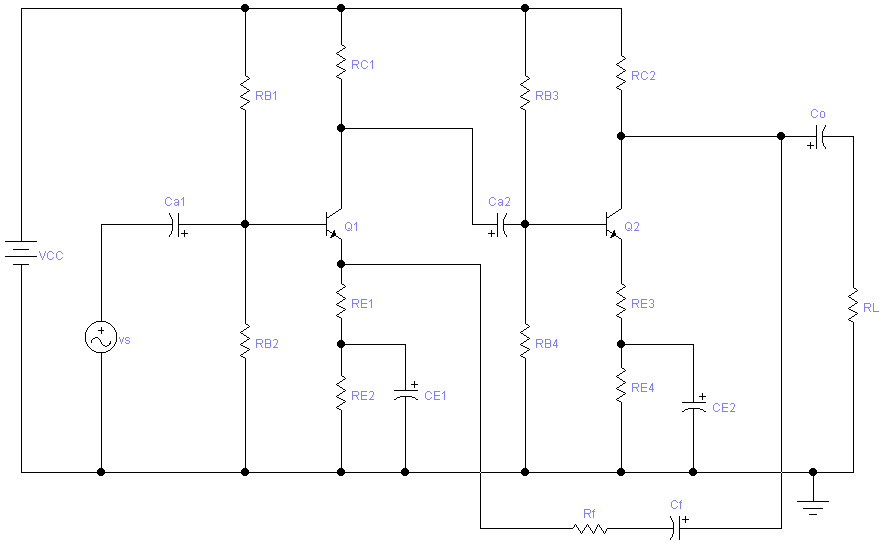
\includegraphics[scale = 0.4]{circuito.png}\\[0.25 cm]	% Imagen Termistor
\caption{Circuito Provisto}
\label{Figura 1}
\end{figure}
\subsection{Componentes}
Lista de componentes:

\begin{tabular}{| l | c || c | c || c | c || c | r | }
 \hline                 
$v_{cc}$ & $22v$ & $r_{e1}$ & $120 \omega$ & $r_f$ & $1.6 k \omega$ & $ c_{e2} $ & $ 10\micro f $ \\
 \hline                 
$r_{b1}$ & $820k\omega$ & $r_{e2}$ & $12k \omega$ & $r_{e3}$ & $240 \omega$ & $ c_{a1} $ & $ 1\micro f $ \\
 \hline                 
$c_{o}$ & $1\micro f$ & $r_{b2}$ & $560k \omega$ & $r_{b3}$ & $120 k \omega$ & $ r_{e4} $ & $ 220\omega $ \\
 \hline                 
$c_{e1}$ & $10\micro f$ & $q_{1}$ & $bc548$ & $r_{c1}$ & $18 k \omega$ & $ r_{b4} $ & $ 22k \omega $ \\
 \hline                
$r_{l}$ & $470\omega$ & $c_{a2}$ & $1\micro f$ & $q_{2}$ & $bc548$ &  &  \\
 \hline  
 \end{tabular}
 
\subsection{Procedimiento}
En primer lugar medimos la ganancia del circuito a lazo cerrado, luego medimos la ganancia del circuito a lazo abierto.

En segundo lugar variamos la resistenia $R_{E2}$ para variar la ganancia de lazo abierto.

En tercer lugar volvimos a medir la ganancia de lazo abierto y confirmamos que hubo un gran cambio en la $\Delta V$.

En cuarto lugar medimos la ganacia de lazo cerrado y observamos la variación de  $\Delta V$.

En quinto lugar con las variaciones anteriores calculamos la desensibilidad.

En sexto lugar procedemos a calcular $Z_O$ y $Z_I$.

En séptimo lugar medimos $Z_O$ y $Z_I$ en el circuito.
\section{Mediciones}
\subsection{Ganancia de tensión }
Para calular la ganacia de tensión del circuito, injectando en la base del primer transistor una señal que no cause
distorsión a la salida del circuito, para asi calcular $\Delta V$.
\begin{equation}
\label{eq:gananciaTension}
\Delta V = \frac{V_O}{V_I} 
\end{equation}
Los valores obtenidos en la mediciones fueron(lazo abierto):

$V_I=280 mV$(Pico a Pico)

$V_O=12 V$(Pico a Pico)

Reemplazando los valores en  \ref{eq:gananciaTension} obtuvimos: 


$\Delta V=40$

Los valores obtenidos en la mediciones fueron(lazo cerrado):

$V_I=570 mV$(Pico a Pico)

$V_{OF}=6.24 V$(Pico a Pico)

Reemplazando los valores en  \ref{eq:gananciaTension} obtuvimos: 

$\Delta V_F=10.94$

\subsubsection{Variacion $R_E$}
Variamos la resistencia del emisor, haciendo que la ganancia de lazo abierto disminuya un $45\textdiscount$
Los valores obtenidos son:
$V_I=128 mV$(Pico a Pico)

$V_O=3.68 V$(Pico a Pico)

Reemplazando los valores en  \ref{eq:gananciaTension} obtuvimos: 

$\Delta V=28$

Esa variacion de la resistencia del emisor provoco un gran cambio en la ganancia de tension en la configuracion de lazo abierto,
pero gracias a la rama de realimentacion la ganancia de lazo cerrado no sufrio un gran cambio.

Los valores obtenidos son:

$V_I=332 mV$(Pico a Pico)

$V_{OF}=3.2 V$(Pico a Pico)

Reemplazando los valores en  \ref{eq:gananciaTension} obtuvimos: 

$\Delta V_F=9.63$

\subsubsection{Calculo de Desensiblidad}
La desensibilidad es un factor que indica la sensiblidad del circuito a los cambios.
\begin{equation}
\label{eq:desensibilidad}
 D = \frac{\Delta \Delta V_f}{\Delta \Delta V}
\end{equation}

Reemplazando en \ref{eq:desensibilidad}:

$D= 0.1091$

\subsection{Impedancia de salida }
La impedancia de salida fue medida colocando un potenciómetro en paralelo a la carga del circuito y variando el mismo de forma tal que la tensión en la carga varé a la mitad. Luego retiramos el potenciómetro y medimos su resistencia con el multímetro.
$ Z_O= 3.55k\Omega$
\subsection{Impedancia de entrada }
La impedancia de entrada fue medida colocando un potenciometro en la entrada del circuito y variándolo de forma tal que la tensión en la salida del circuito varié a la mitad. Luego retiramos el potenciómetro y medimos su resistencia con el multímetro.
$Z_I= 23.71k\Omega$
Tanto la impedancia de entrada como la impedancia de salida con realimentacion no es posible medirlas en el circuito.

\subsection{Curva de respuesta en frecuencia}
\begin{tabular}{| c | c | c | c | c | }
 \hline                 
 F(Hz) & $V_O$ & $V_{OF}$ & $\Delta V$ & $\Delta V_{OF}$  \\
 \hline                 
  1       & 0    & 0    & 0     & 0 \\
 \hline                 
  50      & 1    & 1.28 & 4     & 5.12  \\
 \hline                 
  100     & 7.20 & 1.92 & 28.8  & 7.68  \\
 \hline                
  500     & 8.48 & 2.72 & 33.92 & 10.88  \\
 \hline                
  1000    & 8.68 & 2.8  & 34.56 & 11.2  \\
 \hline                
  2000    & 8.72 & 2.8  & 34.88 & 11.2 \\
 \hline                
  5000    & 8.50 & 2.8  & 34    & 11.2 \\
 \hline                
  10000   & 8.5  & 2.8  & 34    & 11.2 \\
 \hline                
  100000  & 8.8  & 2.8  & 35.2  & 11.2  \\
 \hline                
  200000  & 8    & 2.8  & 32    & 11.2  \\
 \hline                
  500000  & 7.2  & 2.8  & 28.8  & 11.2  \\
 \hline                
  750000  & 6    & 2.8  & 24    & 11.2  \\
 \hline                
  1000000 & 5.20 & 2.8  & 20.8  & 11.2  \\
 \hline                
  2000000 & 2.6  & 2.56 & 10.4  & 12.29  \\
 \hline                
 \end{tabular}

\section{Conclusiones}
Hemos podido observar en el desarrollo del trabajo práctico, las grandes ventajas que posee realimentar un circuito amplificador como el analizado.

Es posible observar la mejora que produce la realimentación en cuanto a la respuesta en frecuencia del circuito, volviéndose mucho mas constante la ganancia del circuito para distintas frecuencias, no debemos olvidarnos de mencionar el hecho de que la realimentación sacrifica un poco de ganancia en el circuito, pero no resulta muy grave ya que estos circuitos poseen una ganancia muy grande, gracias a los grandes valores de hfe de los transistores utilizados.

Otra gran ventaja de la realimentación es el hecho de poder diseñar un circuito que no sufra grandes variaciones, dejando de depender de la ganancia de los distintos trancistores que varía mucho entre componentes de la misma camada de fabricación.

Esta topología de circuito también mejora la impedancia de entrada y salida del amplificador, aumentando la impedancia de entrada y disminuyendo la de salida, acercando así al circuito amplifcador a un amplificador ideal, el cual posee impedancia de entrada infinita y de salida nula. 

\end{document}
